\section{Corpus-Based Convolution} %Contortionist}

With the above building blocks available in modular form, the scene was set for integrating the three approaches, (1) intuitive tactile interaction, (2) descriptor-based corpus navigation, (3) real-time convolution as a means of cross-synthesis, in order to improve on each other's limitations. In other words, there was a desire of timbral richeness, recycled virtuosity, expressive gestural control, subtle multidimensional control, all made possible by a slight abuse of convolution, hijacking it from its usual filtering and room acoustics contexts.

We'll explain in this section the principle and implementation of corpus-based convolution (section~\ref{sec:basic}) and then tackle two problems resulting from its usage in an interactive DMI: 
how to avoid abrupt changes and clicks when grains enter and leave the convolver (section~\ref{sec:set}), and
how to make the scattered bits of sound in the corpus into a smooth map through which the player can navigate (section~\ref{sec:mix}). Preprocessing of the piezo input signal to enhance the sonic outcome is then tackled in (section~\ref{sec:preemph}).

% the method: catart selection, paste into buffer~ for multiconvolve - cool and simple!
\subsection{Basic Realisation}\label{sec:basic}

% % figure with schematics
% \begin{figure}[htb]
% \begin{center}
% 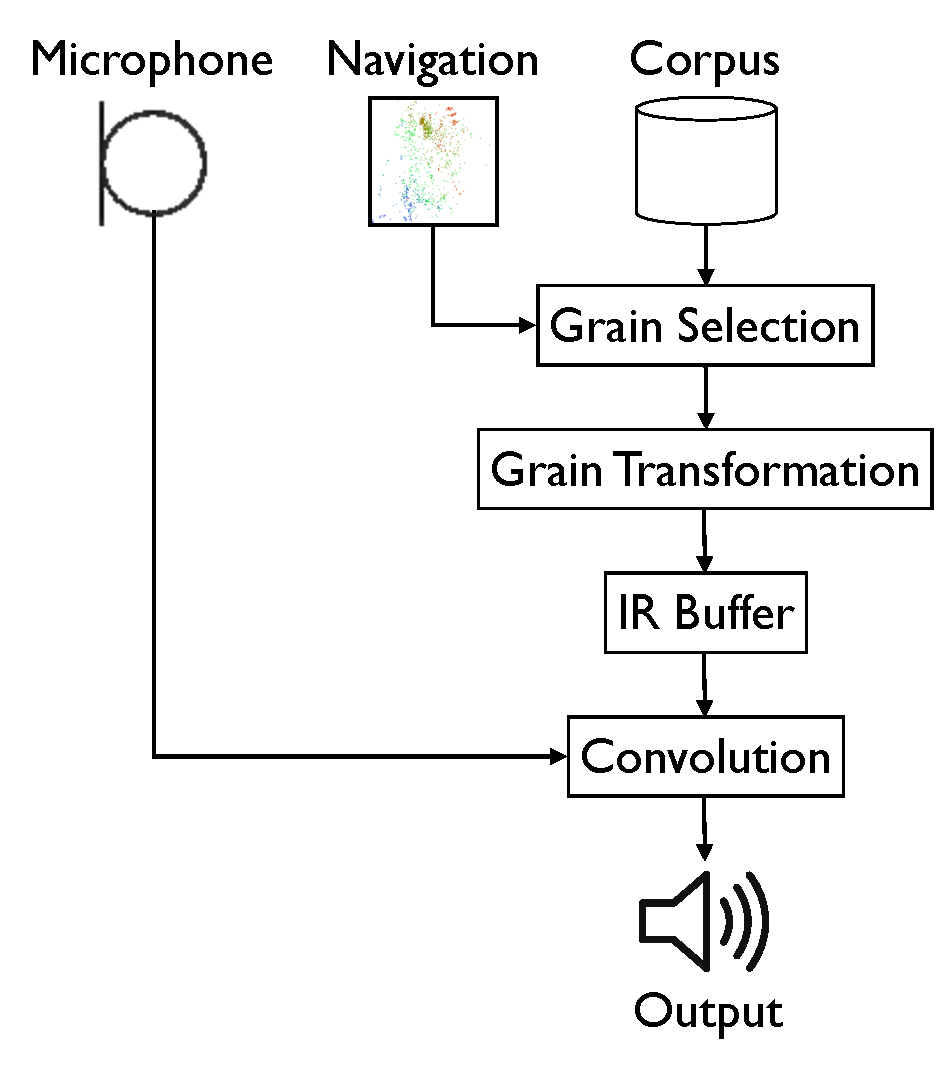
\includegraphics[width=\columnwidth]{pics/flowchart.pdf}
% \caption{Flowchart of the basic realisation of corpus-based convolution.}\label{fig:schema}
% \end{center}
% \end{figure}

The basic realisation of corpus-based convolution is achieved by making a bridge from a selection within the granular \cbcs\ navigator to a convolution engine via an audio buffer, as illustrated in figure~\ref{fig:schema}.  Every time the player navigates in the descriptor space (for instance in a 2D representation as in figure~\ref{fig:corpus}) such that a new grain becomes closest, that grain is taken as an impulse response to be convolved with the microphone input signal. Currently kept in its simplest form, the navigation is done by moving a 2D target via a positional controller such as the mouse, XY-pad (graphics tablet or touch screen) (cf. \cite{Schwarz-nime2012-sound-space}, positional control).

Note that the grain which is used as IR can be processed like any normal grain by the usual time-domain processes, such as transposition, gain, length and envelope change, reversal, all with possible random variations. This further enhances the sonic richness and expressive capabilities of the system.

Technically, in our prototyping system based on \sysname{CataRT}, \sysname{FTM}\footnote{\url{http://ftm.ircam.fr}}, and its  \sysname{Gabor} library, the \code{catart.synthesis} module outputs the grain as a 1-column matrix of floating-point numbers (\code{fmat}).  The matrix is copied into a \verb|buffer~| object via the \code{ftm.buffer} module.
That \verb|buffer~| is referenced by a \verb|multiconvolve~| module from the HISS tools which is notified of the update via a message.

% % figure of corpus
% \begin{figure}[htb]
% \begin{center}
% 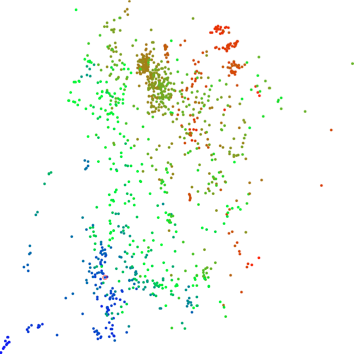
\includegraphics[width=\columnwidth]{pics/schwarz_fig2.png}
% \caption{Example of a corpus projected to 2D for efficient navigation, plotted by Spectral Centroid % (x), Periodicity (y), NoteNumber (colour).}\label{fig:corpus}
% \end{center}
% \end{figure}

% two problems: smooth selection, grain change
The basic realisation above captures the essence of the interaction that allows to choose and then articulate one grain by contact gestures, however it is not yet sufficient for a varied musical performance.  The next three sections will complete the basic realisation to enrich further the sonic outcome.


\subsection{Handling Grain Changes}\label{sec:set}

% polyphony for smooth grain change
When a new grain is selected by navigation in the descriptor space, it is set as a new impulse response for the \verb|multiconvolve~| convolver.  This means that from that moment on, the output signal stops to be the convolution with the old grain, but the one with the new grain, which leads to an abrupt timbral change or even a click.

The aim is to let the old grain ``finish'', while the new grain is already being convolved, in effect reproducing overlap-add mechanism.  This can be achieved by multiplying the convolution modules by means of \maxmsp's \verb|poly~| object.  The old grain's input signal is faded out during a release time of an arbitrary value, in this case 200~ms, which allows the old grain to die out.  Note that the convolution output can still continue for the duration of the grain, so only after $t_r = release time + grain duration$ can the voice be freed.  Simultaneously, a new convolution voice is allocated and receives the new grain and in faded-in by a short attack ramp of 10~ms.

We need a polyphony higher than two, since during the fade out time of one grain, again a new grain can be selected, when the navigation speed in the corpus is fast, or the grains are very dense such that a trajectory crosses several grains within $t_r$. In order not to tax too much the CPU power of the DMI, we have found out thorugh empirical testing that a polyphony of 8 streams was a sufficient compromise between fluid crossfading and CPU usage.

\subsection{Smooth Interpolation Between Grains}\label{sec:mix}

In the basic realisation so far, the navigation in the corpus will switch grains to be convolved as soon as the target position comes closest to a different grain.  
This means the 2D navigation interface is split into discrete Voronoi-polygons.

While for some musical aim this might be appropriate, for instance the creation of rapidly switching timbre transitions, the continuous nature of the navigation space suggests a smoother way to transition between timbres given by the grains in the corpus.

One approach to achieve smooth timbre transitions is to interpolate between the 3 surrounding points in the navigation space.  The relative distances to these points can then be used to derive a weight or amplitude factor \cite{FreedMacCallumSchmederWessel-nime2010-hybridization-interfaces} to mix the convolutions with the 3 grains.  We use this simplified formula to calculate gain factors $g_i$ in dB for $i = 1..3$ convolutions, based on the distances $d_i$ to the 3 closest points:
%
\begin{equation}
  g_i = \frac{g_{min} \, d_i}{d_{min} \sum_{i=1}^3 d_i}
\end{equation}
%
where $g_{min} = -64$~dB is the minimum gain for the maximum distance $d_{min} = \frac{2}{3}$.
The gain for a grain becomes maximum (0 dB) when the target position is on its position, and in the middle of a triangle, all surrounding grain have equal gain.

The implementation needs 3 channels of convolvers of the basic realisation whose output signals are attenuated by $g_i$ and mixed.  They need to be addressed by a channel allocator that keeps grains that don't change in their respective channel, although the order of grain indices in the selection output can change (because it is typically ordered by distance).

\subsection{Pre-Emphasis}\label{sec:preemph}

As the direct signal from the piezo is used to convolve the grains, preprocessing of its sonic characteristics is required: indeed the microphone will exhibit some grain of the surface on which it is applied, most of the time resulting in a dull top-end, with overdynamic spikes when getting too close to the microphone. Moreover, the piezo's high impedance and low gain usually requires high pre-amplifier gains, which is prone to generate background noise. 

We have found that a three band filtering (low high-pass, a band-cut on the main resonance and a boosting high-shelf), followed by a subtle low-threshold expander and a high-threshold limiter, are pre-conditionning the signal and yield results that are much closer to the timbral caracteristics of the IRs selected. By opposition to PUCKETTE, we did not want to loose all the sustaining spectro-morphological qualities of the performing surface, captured in the piezo signal, as we consider that the complex filter offered by this signal is part of the instrument's sound. Nevertheless, the modularity of the current implementation would easily allow the pre-emphasis filtering to be replaced by a FIR-filter extrapolated from inverted surface resonance, as proposed by PUCKETTE.